\section{Résultats numériques}

  \begin{figure}[!hbt]
    \centering
    \tikzsetnextfilename{SER_mono_cone_11352_elt.TM}
\begin{tikzpicture}[scale=1]
    \begin{axis}[
            title={Polarisation TM},
            ylabel={SER (dB)},
            xlabel={\(\theta_{inc}\) (deg)},
            width=0.4\textwidth,
            xmin=0,
            xmax=180,
            ymin=-30,
            ymax=10,
            restrict y to domain=-30:30,
            mark repeat=20,
            legend pos=outer north east
        ]
        \addplot [color=black,mark=square*] table [col sep=comma, x={theta}, y={reference}] {csv/SER/ser_mono_cone_11352_elt.TM.csv};
        \addplot [color=\ccio,mark=x] table [col sep=comma, x={theta}, y={CI0}] {csv/SER/ser_mono_cone_11352_elt.TM.csv};
        \addplot [color=\ccit,mark=diamond*] table [col sep=comma, x={theta}, y={CI3}] {csv/SER/ser_mono_cone_11352_elt.TM.csv};
        \addplot [color=\ccitc,mark=+] table [col sep=comma, x={theta}, y={CI3+CSU}] {csv/SER/ser_mono_cone_11352_elt.TM.csv};
    \end{axis}
\end{tikzpicture}
\tikzsetnextfilename{SER_mono_cone_11352_elt.TE}
\begin{tikzpicture}[scale=1]
    \begin{axis}[
            title={Polarisation TE},
            ylabel={},
            xlabel={\(\theta_{inc}\) (deg)},
            width=0.4\textwidth,
            xmin=0,
            xmax=180,
            ymin=-25,
            ymax=10,
            restrict y to domain=-25:10,
            mark repeat=20,
            legend pos=outer north east
        ]
        \addplot [color=black,mark=square*] table [col sep=comma, x={theta}, y={reference}] {csv/SER/ser_mono_cone_11352_elt.TE.csv};
        \addlegendentry{Référence};
        \addplot [color=\ccio,mark=x] table [col sep=comma, x={theta}, y={CI0}] {csv/SER/ser_mono_cone_11352_elt.TE.csv};
        \addlegendentry{CI0};
        \addplot [color=\ccit,mark=diamond*] table [col sep=comma, x={theta}, y={CI3}] {csv/SER/ser_mono_cone_11352_elt.TE.csv};
        \addlegendentry{CI3};
        \addplot [color=\ccitc,mark=+] table [col sep=comma, x={theta}, y={CI3+CSU}] {csv/SER/ser_mono_cone_11352_elt.TE.csv};
        \addlegendentry{CI3\textsubscript{CSU}};
    \end{axis}
\end{tikzpicture}
    \caption[SER monostatique d'un cône-sphère calculée par un code EI]{\(\eps = 1 - i\), \(\mu = 1\), \(d = 5\)cm, \( f =  200\) MHz, maillé \(\lambda_0/55\), \(\theta_{obs}=\theta_{inc}\)}
    \label{fig:ser:cone-sphere-mono-M1}
  \end{figure}

  La figure \ref{fig:ser:cone-sphere-mono-M1} contient la SER monostatique d'un cône-sphère, éclairé depuis le nez, calculée par un code de référence , calculée par un code axis symétrique de type équations intégrales avec éléments finis avec maillage des matériaux et cette SER est comparée avec les SER calculées par le code maquette équations intégrales couplées avec les CIOE CI0 et CI3 où les coefficients sont calculés dans le cadre de l'approximation du plan tangent.

  \begin{figure}[!hbt]
    \centering
    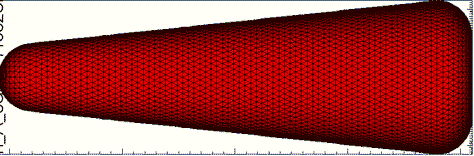
\includegraphics[width=0.8\textwidth]{images/cone.png}
    \caption{Cône-sphère de longueur 2 mètres et de demi-angle 8 degrés maillé avec 11352 éléments.}
    \label{fig:obj:cone-sphere}
  \end{figure}

  Il y a 34056 inconnus pour le système linéaire final, pour ce cône-sphère (voir figure \ref{fig:obj:cone-sphere}).
  Avec une structure de données type matrice complexe pleine sur 64 bits, cela représente au moins 19 Go de mémoire pour le système linéaire seul, et au moins 28 Go cumulativement pour les sous-matrices.

  % \begin{remark}
  %   La surface étant régulière sans bords, le nombre d'inconnus total est \(N_{éléments}*3/2*2\), \(3/2\) correspondant au rapport arêtes/élements, et \(2\) car pour chaque arête, il y a une inconnue pour chaque champ \(\vE,\vH\).
  %   Les tailles mémoire en bits des matrices sont alors \(N_{inconnus}^2*2*N_{bits}\), le facteur 2 correspond au stockage de la partie réelle et imaginaire.
  % \end{remark}

  \FloatBarrier

  \begin{figure}[!hbt]
    \centering
    \tikzsetnextfilename{SER_bis_sphere_4240_elt.TM}
\begin{tikzpicture}[scale=1]
    \begin{axis}[
            title={Polarisation TM},
            ylabel={SER (dB)},
            xlabel={\(\theta_{obs}\) (deg)},
            width=0.4\textwidth,
            xmin=0,
            xmax=180,
            ymin=-27,
            ymax=25,
            restrict y to domain=-30:30,
            mark repeat=20,
            legend pos=outer north east
        ]
        \addplot [color=black,mark=square*] table [col sep=comma, x={theta}, y={Mie}] {csv/SER/ser_bis_sphere_4240_elt.TM.csv};
        \addplot [color=\ccio,mark=x] table [col sep=comma, x={theta}, y={CI0}] {csv/SER/ser_bis_sphere_4240_elt.TM.csv};
        \addplot [color=\ccit,mark=diamond*] table [col sep=comma, x={theta}, y={CI3}] {csv/SER/ser_bis_sphere_4240_elt.TM.csv};
        \addplot [color=\ccitc,mark=+] table [col sep=comma, x={theta}, y={CI3+CSU}] {csv/SER/ser_bis_sphere_4240_elt.TM.csv};
    \end{axis}
\end{tikzpicture}
\tikzsetnextfilename{SER_bis_sphere_4240_elt.TE}
\begin{tikzpicture}[scale=1]
    \begin{axis}[
            title={Polarisation TE},
            ylabel={},
            xlabel={\(\theta_{obs}\) (deg)},
            width=0.4\textwidth,
            xmin=0,
            xmax=180,
            ymin=0,
            ymax=20,
            restrict y to domain=0:25,
            mark repeat=20,
            legend pos=outer north east
        ]
        \addplot [color=black,mark=square*] table [col sep=comma, x={theta}, y={Mie}] {csv/SER/ser_bis_sphere_4240_elt.TE.csv};
        \addlegendentry{Mie};
        \addplot [color=\ccio,mark=x] table [col sep=comma, x={theta}, y={CI0}] {csv/SER/ser_bis_sphere_4240_elt.TE.csv};
        \addlegendentry{CI0};
        \addplot [color=\ccit,mark=diamond*] table [col sep=comma, x={theta}, y={CI3}] {csv/SER/ser_bis_sphere_4240_elt.TE.csv};
        \addlegendentry{CI3};
        \addplot [color=\ccitc,mark=+] table [col sep=comma, x={theta}, y={CI3+CSU}] {csv/SER/ser_bis_sphere_4240_elt.TE.csv};
        \addlegendentry{CI3\textsubscript{CSU}};
    \end{axis}
\end{tikzpicture}
    \caption[SER bistatique d'une sphère calculée par un code EI]{\(\eps = 1 - i\), \(\mu = 1\), \(d = 5\)cm, \( f =  200\) MHz, maillé \(\lambda_0/18\), \(\theta_{inc}=0\)}
    \label{fig:ser:sphere-bis-M1}
  \end{figure}

  La figure \ref{fig:ser:sphere-bis-M1} contient les SER bistatique d'une sphère par équations intégrales couplées avec les CIOE CI0 et CI3 où les coefficients sont calculés dans le cadre de l'approximation du plan tangent, et ces SER sont comparées avec celle obtenue par série de Mie.

  Par manque de temps, nous n'avons pas de résultats numériques avec des coefficients de CIOE calculés avec le cas du cylindre ou de la sphère.

  Ces figures montrent que la SER calculée par EI avec CIOE est très proche de la solution de référence, même dans l'approximation du plan tangent et valident numériquement notre méthode.

  \FloatBarrier